\documentclass{article}
\IfFileExists{iclr2027_conference.sty}{\usepackage{iclr2027_conference}}{\usepackage[margin=0.82in]{geometry}}
\usepackage{amsmath,amssymb,amsthm,booktabs,graphicx,hyperref,microtype,xcolor,array,tabularx}
\graphicspath{{figures/}}
\newtheorem{theorem}{Theorem}
\newtheorem{proposition}{Proposition}
\newcommand{\PendingCell}{\textcolor{red!75!black}{\texttt{PENDING}}}
\newcommand{\ResultPending}[1]{\textcolor{red!75!black}{\texttt{RESULT\_PENDING[#1]}}}
% Use a vector Computer Modern glyph for first-level list markers.  The
% default text bullet can become a Type 3 bitmap under the fallback article
% build, which is unsuitable for an archival manuscript.
\renewcommand{\labelitemi}{\ensuremath{-}}
\setlength{\emergencystretch}{2em}
\title{Supplement: CoReGraph under Compositional Deployment Contracts}
\author{Anonymous Authors}
\begin{document}
\maketitle
\noindent\textbf{Status: RESULTS\_BLOCKED.} This supplement contains proofs, implementation and benchmark details, the frozen statistical plan, empty result templates, reproducibility information, and a checklist. It contains no real Level-4 metric.
\section{Proofs and counterexamples}

\subsection{Fixed-mixture impossibility}
\begin{theorem}
For risks \((0,\delta_1)\) and \((\delta_2,0)\) with \(\delta_1,\delta_2>0\), any contract-independent randomized expert selector has minimax regret \(\delta_1\delta_2/(\delta_1+\delta_2)\), whereas a contract-aware selector has zero regret.
\end{theorem}
\begin{proof}
Let \(w\in[0,1]\) be the probability of expert one. By affine randomized-selection risk, contract regrets are \(r_1(w)=(1-w)\delta_1\) and \(r_2(w)=w\delta_2\). The first decreases and the second increases. Their maximum is minimized at their unique intersection; otherwise moving toward the intersection reduces the larger term. Solving gives \(w^\star=\delta_1/(\delta_1+\delta_2)\), and substitution gives the stated positive value. Conditioning on the contract chooses the zero-risk expert in each environment.
\end{proof}
If a resource mask changes the feasible set, the same argument applies to the two feasible risk gaps when their optima reverse. If either gap vanishes or one feasible expert is optimal everywhere, a positive lower bound does not follow. Prediction averaging under nonlinear loss is outside the affine selection premise.

\subsection{Regret decomposition}
Let \(\pi^{(0)}\) be the ideal policy and \(\pi^{(1)},\ldots,\pi^{(7)}=\hat\pi\) successively replace representation, diagnostics, router approximation, feasible set, budget, abstention, and population risk with deployed counterparts. Adding and subtracting adjacent risks yields
\[
R_c(\hat\pi)-R_c(\pi^{(0)})=\sum_{k=1}^{7}\left[R_c(\pi^{(k)})-R_c(\pi^{(k-1)})\right].
\]
Taking absolute values and applying the triangle inequality gives the stated sum of nonnegative errors. The identity does not imply the intermediate contrasts are identifiable from observational target data; it specifies proof obligations and diagnostic counterfactuals.

\subsection{Compositional approximation}
\begin{theorem}
Suppose \(R(a,c)=b(a)+\sum_jf_j(a,c_j)+h(a,c)\), \(|h|\leq\epsilon_{\mathrm{int}}\), and \(|\hat f_j-f_j|\leq\epsilon_j\) uniformly for source-observed values. If \(\hat a\) is within \(\epsilon_{\mathrm{route}}\) of the minimizer of the estimated additive risk, then on any unseen combination of those values,
\[
R(\hat a,c)-R(a^\star,c)\leq 2\sum_j\epsilon_j+2\epsilon_{\mathrm{int}}+\epsilon_{\mathrm{route}}.
\]
\end{theorem}
\begin{proof}
Let \(\hat R_0(a,c)=b(a)+\sum_j\hat f_j(a,c_j)\). For every action, \(|R(a,c)-\hat R_0(a,c)|\leq\sum_j\epsilon_j+\epsilon_{\mathrm{int}}=:\epsilon\). Thus
\[
R(\hat a,c)\leq\hat R_0(\hat a,c)+\epsilon
\leq\hat R_0(a^\star,c)+\epsilon_{\mathrm{route}}+\epsilon
\leq R(a^\star,c)+2\epsilon+\epsilon_{\mathrm{route}}.
\]
\end{proof}
An XOR risk over two binary axes has zero marginal main effects but a nonzero joint term; without a bounded interaction residual, a factorized predictor cannot identify the unseen corner from the marginals.

\subsection{Mask and selective-risk results}
For a nonempty feasible set, exponentiating \(-\infty\) gives zero and normalizing the finite feasible exponents gives unit mass. Every selected expert satisfies the conjunction defining the mask. The empty-set branch is defined separately and therefore does not invoke softmax on all \(-\infty\) logits.

For selective risk, the density-ratio assumption gives
\(\mathbb E_t[\ell\mathbf 1_A]\leq\kappa\mathbb E_s[\ell\mathbf 1_A]=\kappa P_s(A)R_s^{\mathrm{sel}}\).
Dividing by \(P_t(A)\geq\gamma\) and using bounded loss gives the claimed minimum with \(L\). If \(\gamma=0\), conditional risk is undefined.

\subsection{Executable finite failures}
The artifact checks protocol one-hot memorization, crossing mixtures, overconfident wrong experts, hidden masks, wrong cross-dataset seed pairing, runtime/latency substitution, noisy-contract non-identifiability, XOR interactions, and zero-coverage semantics. Passing these checks confirms each finite construction, not real-data assumptions.

\section{Implementation details}

The contract schema accepts exactly six axes. Each observation stores a category or continuous value, state (`observed`, `missing`, `uncertain`, `out\_of\_range`, `unseen`), and confidence. Source-only statistics normalize continuous axes; zero-variance scales become one. Category vocabularies reserve missing and unknown indices. Encoder manifests record dimensions, vocabulary, normalization authority, pairwise interactions, and attention.

The hierarchical router uses a two-layer contract head and two-layer instance-correction head. Tanh bounds corrections; an optional magnitude threshold makes them sparse. Contract-only sets corrections to zero, and instance-only removes the prior. The mask composes availability, memory, latency, and invocation predicates as aligned batch-by-expert tensors. All-unavailable rows emit zero weights and expert sentinel \(-1\).

Diagnostics are modular declarations. Source calibration fits only source validation; feature drift fits source-train moments; graph statistics use only the admissible visible graph. Missing values carry masks and confidence rather than silent zeros. The optional latent discovery head cannot be constructed unless an experimental flag is set.

Objective terms are normalized as source group means. The feasible oracle is computed after expert losses are aggregated per contract. CVaR averages the worst empirical contract tail. Review surrogates are computed within constrained source groups. Resource records distinguish measured, estimated, and unknown quantities. Run manifests are created before execution and existing coordinates are skipped only after hash validation.

\begin{figure}[t]
  \centering
  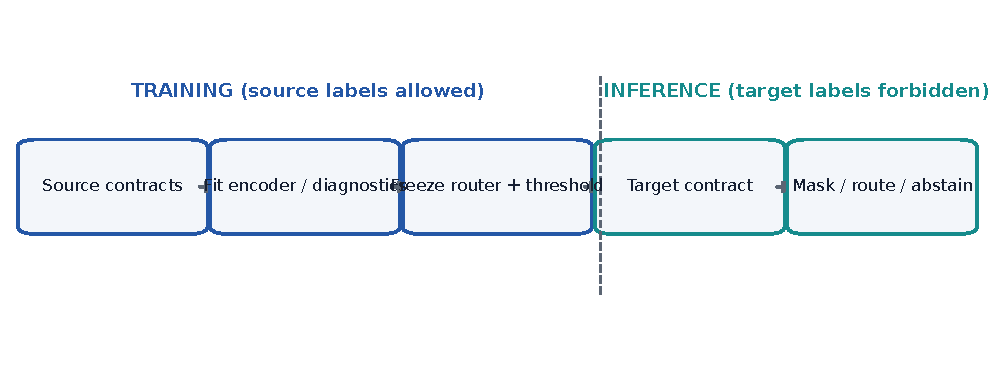
\includegraphics[width=\linewidth]{04_training_inference_flow.pdf}
  \caption{Source-only fitting and target-label-free inference boundary.}
\end{figure}

\section{Benchmark and scenario details}

The saved-output V5 grid is \(2\) datasets \(\times 3\) protocols \(\times 3\) experts \(\times 10\) seeds, yielding 180 role-neutral coordinates. Each dataset, target protocol, and seed defines one held-out scenario, yielding 60 scenarios. Each scenario binds two source protocols times three experts and one target protocol times three experts: six source and three target bindings, or 540 total.

Source bindings permit train and validation rows; target bindings permit known-label test rows for evaluation only. Target protocol is absent from sources, target labels are unavailable during fitting, and one base coordinate cannot have both roles within a scenario. Byte-backed checks additionally require disjoint row scopes, valid chronology, exact dataset and seed identity, provider-label/score alignment, and exclusion of unknown labels.

The six archive names and expected hashes live in the evidence manifest. No filename-only substitution is accepted. The archive reader verifies the complete ZIP and member hashes by streaming, validates schema, filters split and label-known rows, and never exposes permanent extraction.

Controlled mechanisms have tiny deterministic fixtures and future pilot/full modes. Expected router directions are qualitative sanity checks only where the mechanism construction entails them. GOOD is primary for non-fraud graph OOD; official installation, licence, task bridge, and parity remain separate gates.

\section{Frozen statistical plan}

The primary paired unit is dataset, held-out target contract, and expert-prediction seed. Analyses are separate per fraud dataset. Exact Wilcoxon and paired permutation tests, raw paired differences, robust standardized effects, and seed-block bootstrap 95\% intervals are reported. Holm correction applies within each frozen claim family. A dataset-seed hierarchical bootstrap is secondary.

Missing cells are not imputed. Integrity-invalid cells are excluded with reason; resource-blocked cells restrict the common comparison set. The frozen primary comparisons are uniform averaging, best fixed expert, source logistic/MLP gates, strongest feasible graph-MoE, and strongest feasible graph-OOD. Oracle diagnostics do not enter deployable comparison families.

A pilot GO requires complete integrity and leakage gates, directional improvement over uniform averaging, lower worst-contract regret on both fraud datasets, no practically concerning primary reversal, exact mask behavior, useful nonzero abstention coverage, seed stability, and no target-label/oracle input. The preregistration hash is stored in the build report before real results.

\section{Additional result templates}

\begin{itemize}
  \item \ResultPending{S1-REGRET} and \ResultPending{S2-BUDGET}.
  \item \ResultPending{S3-ROUTING} and \ResultPending{S4-COUNTERFACTUAL}.
  \item \ResultPending{S5-LATENT}.
\end{itemize}

The following figures are deliberately empty. They establish labels and layout without curves, points, heatmap values, or implied ordering.

\begin{figure}[h]
\centering
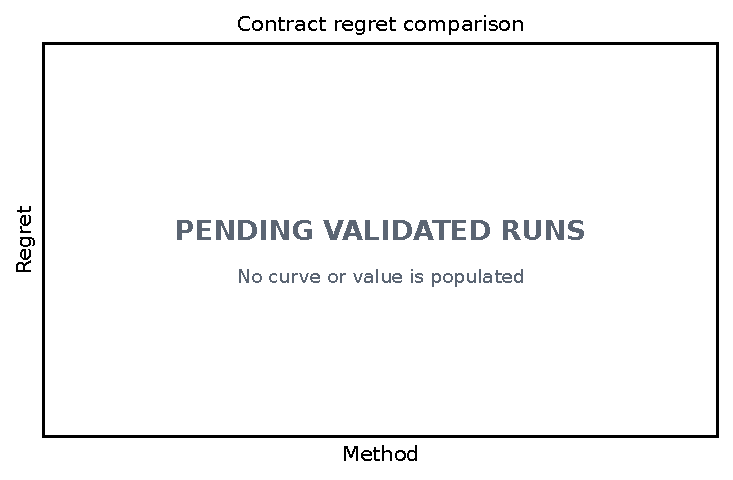
\includegraphics[width=.48\linewidth]{template_regret_comparison.pdf}\hfill
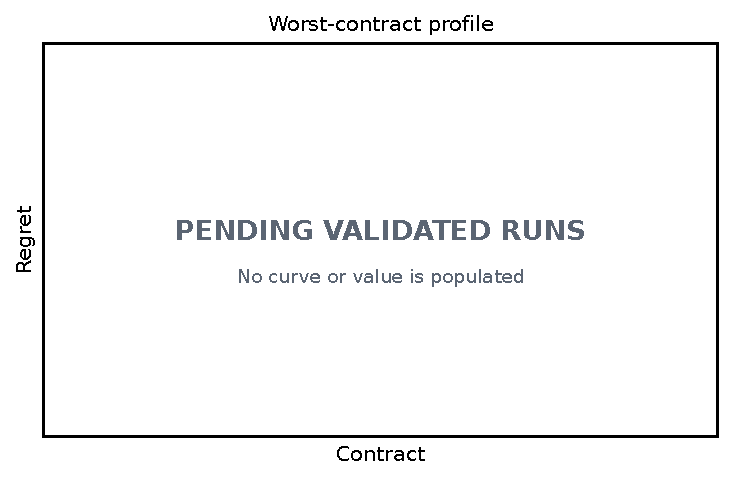
\includegraphics[width=.48\linewidth]{template_worst_contract.pdf}
\caption{Blocked regret templates.}
\end{figure}
\begin{figure}[h]
\centering
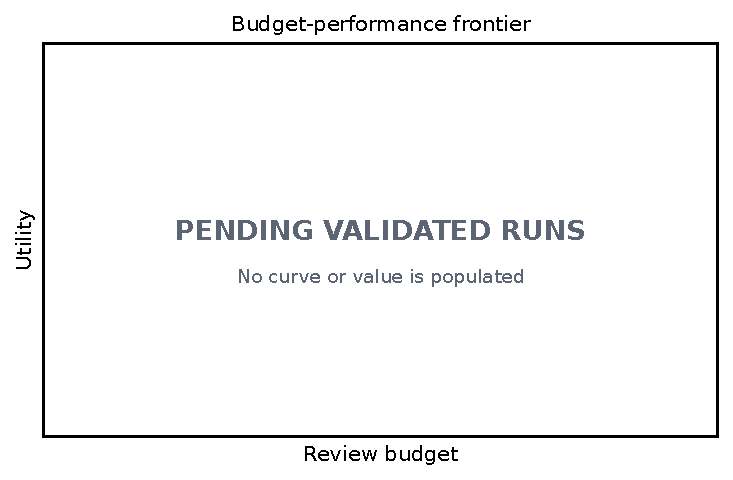
\includegraphics[width=.48\linewidth]{template_budget_frontier.pdf}\hfill
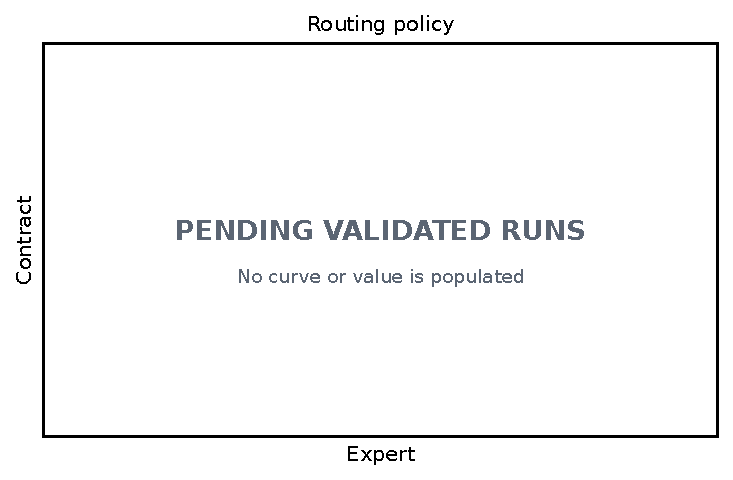
\includegraphics[width=.48\linewidth]{template_routing_heatmap.pdf}
\caption{Blocked budget and routing templates.}
\end{figure}
\begin{figure}[h]
\centering
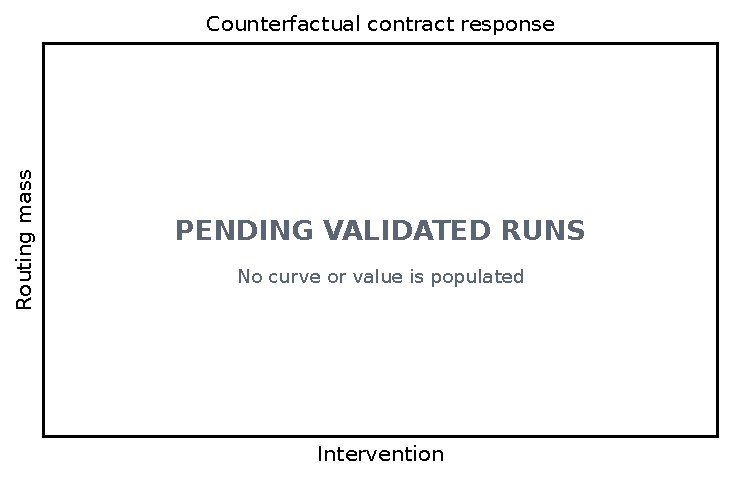
\includegraphics[width=.48\linewidth]{template_counterfactual.pdf}\hfill
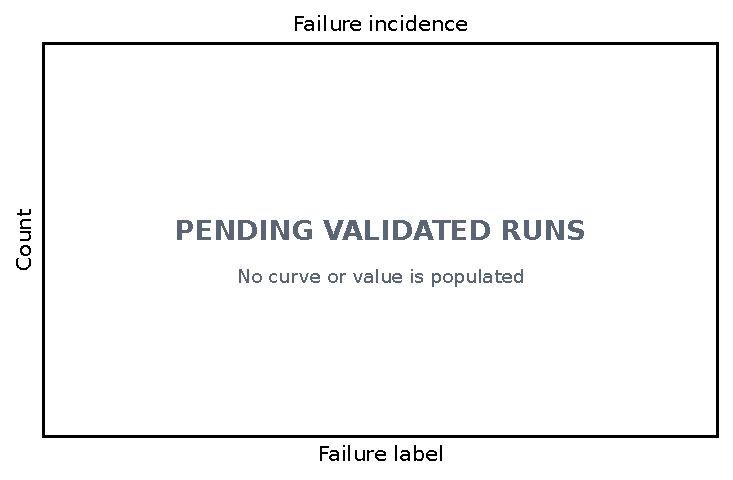
\includegraphics[width=.48\linewidth]{template_failure_taxonomy.pdf}
\caption{Blocked counterfactual and failure templates.}
\end{figure}
\begin{figure}[h]
\centering
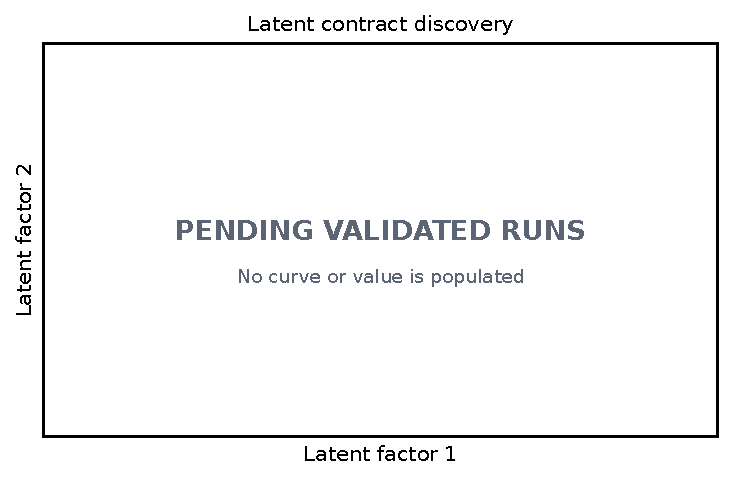
\includegraphics[width=.52\linewidth]{template_latent_contract.pdf}
\caption{Blocked latent-contract template.}
\end{figure}

No text may replace these tokens until the result importer validates code/config/data/prediction hashes, completeness, exclusion reasons, claim linkage, and the frozen statistical gate.

\section{Reproducibility and release}

\begin{table*}[t]
\centering
\caption{Build-phase reproducibility status.}
\label{tab:reproducibility}
\small
\begin{tabular}{lll}
\toprule
Item & Status & Boundary \\
\midrule
Contract, router, objective, mechanism code & available & deterministic tiny tests \\
Run and claim matrices & frozen & no real result observed \\
Six canonical archives & verified local cache & no payload redistributed \\
Official baselines & not installed & licence/parity gates retained \\
Paper empirical cells & blocked & no fabricated number \\
Anonymous source release & clean-room validated & provider data excluded \\
\bottomrule
\end{tabular}
\end{table*}


Every future run emits code SHA, canonical configuration and hash, data/archive/member hashes, environment, prediction hash, resource measurement, validation, completeness, exclusion reason, and claim linkage. Coordinates are resumable only after hash equivalence. The full matrix is frozen as plan rows with unknown runtime and memory rather than fabricated estimates.

Source snapshots exclude Git metadata, environments, caches, data, predictions, checkpoints, private paths, logs, and LaTeX intermediates. The clean-room test extracts a snapshot, installs or selects a fresh environment, runs tiny gates, builds both PDFs, scans for private path/identity, validates release checksums, and verifies the frozen inherited boundary. Data or outputs with unresolved licences are not published.

The evidence cache is outside Git. All six canonical archives, 180 prediction-member identities and hashes, schemas, coordinates, chronology, label-known semantics, 60 cross-expert alignment groups, and 20 cross-protocol dataset-seed row scopes pass through streaming audits without permanent extraction or SSD access. This closes pilot-input integrity, not empirical evaluation: no pilot metric or oracle has been computed.

\section{Submission checklist}

\begin{itemize}
  \item Claims distinguish theory, build validation, and empirical evidence: \textbf{yes}.
  \item Assumptions and counterexamples accompany theory: \textbf{yes; external mathematical review pending}.
  \item Numerical Level-4 results fabricated: \textbf{no}.
  \item Target labels used for fitting or threshold selection: \textbf{no execution occurred}.
  \item Official baselines installed or represented as integrated: \textbf{no}.
  \item Provider data or prediction payload redistributed: \textbf{no}.
  \item Resource measurements available: \textbf{no; blocked}.
  \item Frozen FraudShiftBench/TKDE scientific files changed: \textbf{must remain zero under final gate}.
  \item Main and supplement anonymous: \textbf{automated scan required after build}.
  \item Target-year ICLR template and policy verified: \textbf{blocked; no official 2027 template found at build time}.
  \item LLM-use disclosure completed for target venue: \textbf{policy check and author completion required}.
\end{itemize}

The paper is not submission-ready while empirical, official-baseline, resource, external-review, template, and final packaging gates remain open.

\bibliographystyle{plain}
\bibliography{references}
\end{document}
